\documentclass[11pt,a4paper]{article}

\usepackage[utf8]{inputenc}
\usepackage{graphicx}
\usepackage{float}
\usepackage[singlespacing]{setspace}
\usepackage[left=2.5cm,right=2.5cm,top=2cm,bottom=2cm]{geometry}

\setlength{\parskip}{5pt plus 1 pt minus 1 pt}

\begin{document}

\thispagestyle{empty}
\pagestyle{empty}

{\bf\centerline{{\huge CV}}}
\vspace{6pt}

\centerline{Adrian Regenfuß (*28.10.1997)}
\centerline{Weinschenkstraße 4a}
\centerline{80999 Munich, Allemagne}
\centerline{+49-89-80 92 86 94}
\centerline{a.regenfuss@gmx.de}
\smash{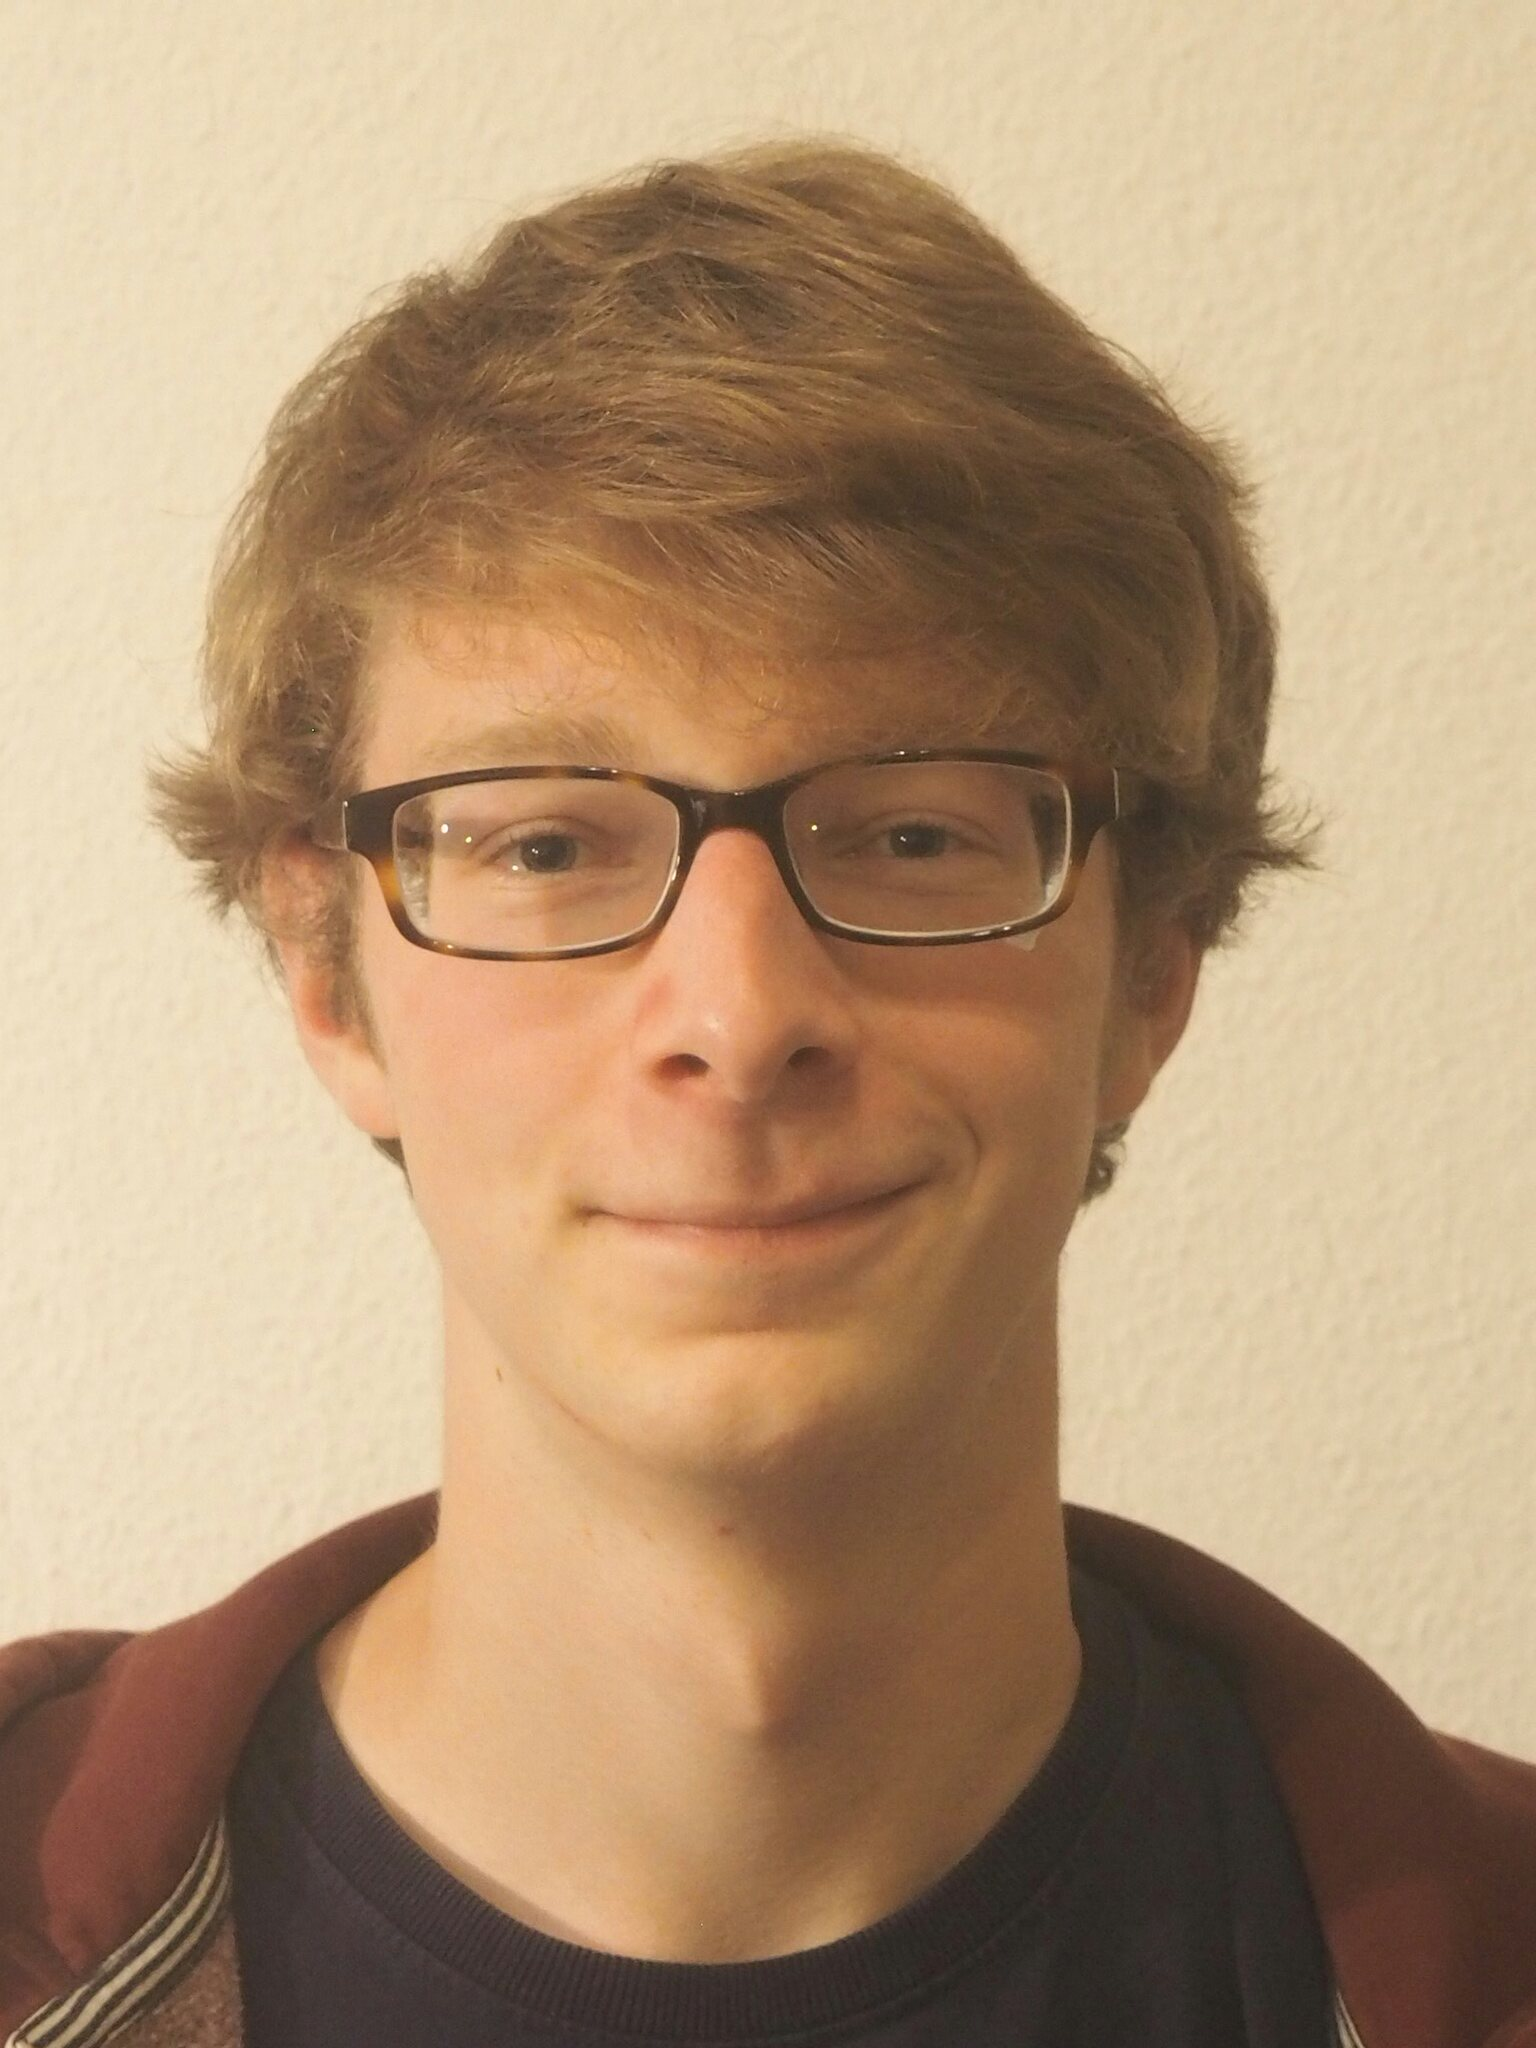
\includegraphics[scale=0.3]{./farbe.jpg}}

\vspace{5pt}

Je suis un étudiant curieux, motiveé, et ambitieux à apprendre des technologies
et logiciels nouvelles. J'ai une experience personelle en faire de la programmation
et en administrer des systemes unix. Je suis aussi curieux par apprendre plus
du design des logiciels professionel et des nouvelles methodes du development.

J'ai fini college été 2016 avec des grades excellentes. Au moment je fais mes études
en physique, mais j'envisage de passer à informatique en automne de 2017. Avant, je voudrais
bien gagner de l'experience practical et internationale.

\section*{Compétences techologiques}
\begin{itemize}
	\setlength{\itemsep}{1pt}
	\item[]{\bf Languages}: C/C++, Bash, Java, Lua, Visual Basic, Miranda
	\item[]{\bf Système opérateur}: Unix, Windows, Plan 9 from Bell labs
	\item[]{\bf outils}: git, make, gdb, awk, sed, regular expressions, Code::Blocks, LaTeX
	\item[]{\bf base de donneés2}: SQL
\end{itemize}

\section*{Historique de l'emploi}
\begin{itemize}
	\setlength{\itemsep}{1pt}
	\item Stage au Deep Learning Competence Center dans le centre allemand pour la recherche de l'intelligence artificielle
	(Deutsches Forschungszentrum für Künstliche Intelligenz, www.dfki.de), avec un accent sur l'analyse des données visuelles en utilisant des des réseaus neuronales.\\
	\hfill Septembre - Novembre 2016
	\item Emploi d'été à Allocation Network GmbH en Munich (entretien d'un logiciel et essai d'un système commerciel pour la gestion des fournisseurs)
	\hfill Juin et Juillet 2016
	\item Stage à Allocation Network GmbH en Munich (projet de trouver
	\& eliminer des emails dupliqueés dans le exchange mail server de l'entreprise - conception, construction et essai)
	\hfill Juin 2014
	\item Stage à la Maison de vente aux enchères Karl \& Faber in Munich \hfill Juillet 2013, Novembre 2013
\end{itemize}

\section*{Projets logiciels récents}
\begin{itemize}
	\setlength{\itemsep}{1pt}
	\item Un client pour le protocol distribué tox utilisant un système de fichiers\\
	(git.z3bra.org/ratox/log.html)
	\item Logiciel pour la generation d'un dictionnaire avec des fréquences des mots
	par analyzer des pages de Wikipedia
	\item Génération des chaînes en systèmes formels à haute performance
	(basé sur Douglas Hofstadter's ''MU``)
	\item Contributions aux projets open source ogg122 (github.com/dimkr/ogg122),\\
	sbase (git.suckless.org/sbase) et human (git.z3bra.org/human/log.html)
	\item Plus des projets à github.com/pranomostro
\end{itemize}

\section*{Éducation}
\begin{itemize}
	\setlength{\itemsep}{1pt}
	\item[] Études en physique à l'université technologique de munich \hfill Depuis septembre 2016
	\item[] École secondaire, fini avec le bac (Allemand Abitur).
	Grade finale de 1.5 sur une échelle de 1 à 6, où 1 est la meilleure marque. Karlsgymnasium Pasing, Bavière.
	\hfill Février 2012 - Juin 2016
	\item[] 2 semaine language échange à Clermont-Ferrand, France
	\hfill Juin 2013, Avril 2014
	\item[] Fini un échange d'une semaine à Broadstairs, Angleterre \hfill Juillet 2012
	\item[] Kaiserin Friedrich Gymnasium à Bad-Homburg, land de Hesse \hfill 2008 - 2012
	\item[] Peter-Härtling Schule à Friedrichsdorf, land de Hesse \hfill 2004 - 2008
\end{itemize}

\section*{Activiteés périscolaires}
\begin{itemize}
	\setlength{\itemsep}{1pt}
	\item[] Co-création d'un guide audio pour un camp de travail allemand historique près de Munich
	\hfill Mars 2016
	\item[] Dépensé une période à Scotch College, Melbourne \hfill Julliet - Septembre 2014
	\item[] Échange d'étude d'anglais de 2 semaines à Melbourne, Australie \hfill Août 2013
\end{itemize}

\section*{Capacités supplémentaires}
\begin{itemize}
	\setlength{\itemsep}{1pt}
	\item Parler et écrire d'anglais couramment
	\item Lire et parler du français couramment (level B1)
	\item Dactylographie avec 70 mots par minute
\end{itemize}

\section*{Intérêts}
\begin{itemize}
	\setlength{\itemsep}{1pt}
	\item Programmation
	\item Projets de la software open source
	\item Algorithmes et apprentissage automatique
	\item Taek-Won-Do
	\item Jouer du piano, de la clarinette and du saxophone baryton
	\item Philosophie
\end{itemize}

\section*{Références}
Andreas Vollmann, Director - Allocation Network GmbH Munich (mail@allocation.net)

\end{document}
